\subsection{Application to radio relics}
\label{sec:results_relics}

In order to test the model's response to the isolated diffuse emission, we apply the \(50\)-member ensemble to the ten selected, polygon-masked relic cutouts listed in Table~\ref{tab:relic_sample}. Detailed preprocessing is described in Sec.~\ref{sec:method_relics}.
Figure~\ref{fig:relic_grid} shows the actual inputs. Identification of relics in unmasked survey fields using an automated approach is a challenging task and lies beyond the scope of this work.

\begin{figure}[H]
\centering
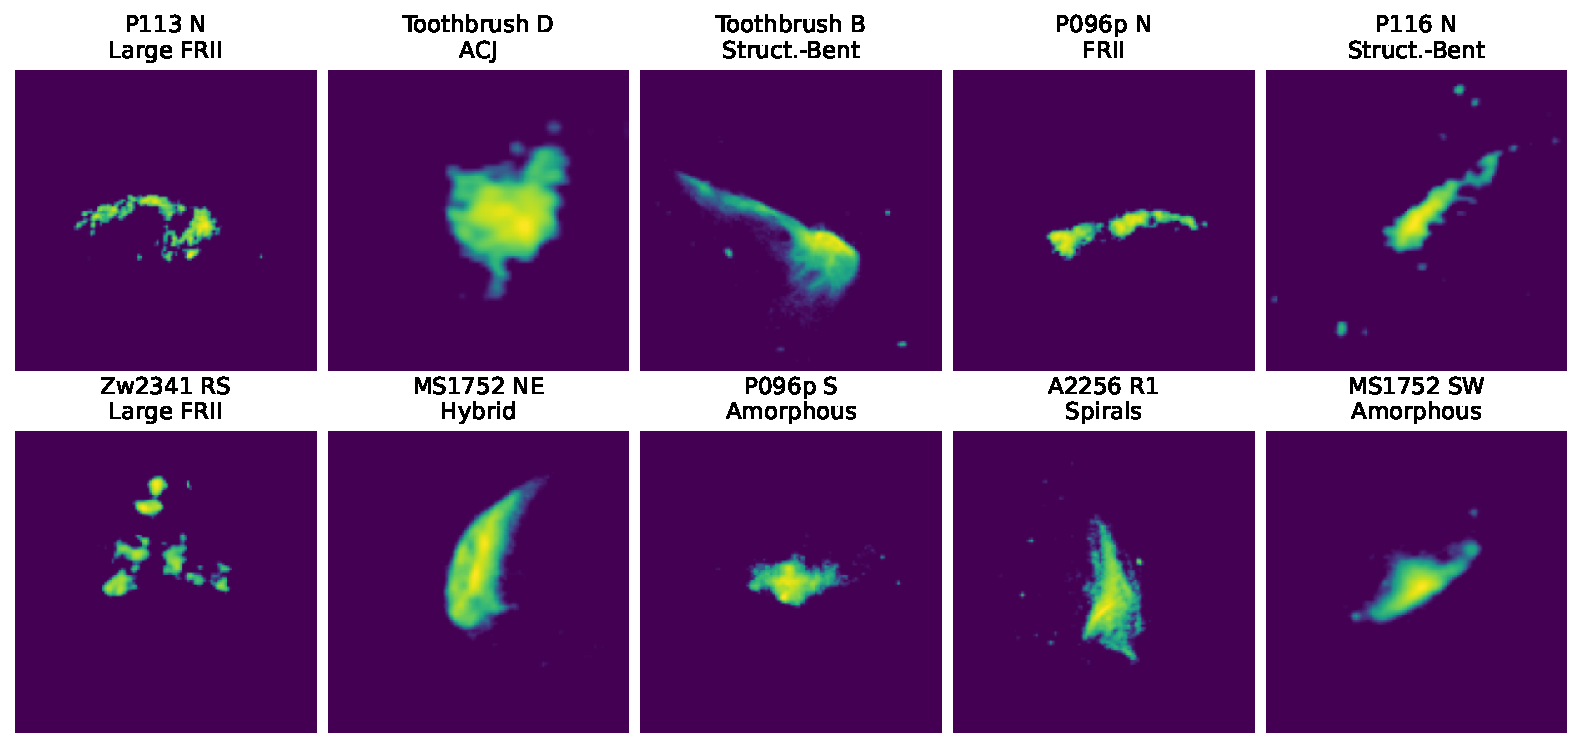
\includegraphics[width=\linewidth]{img/relic_image_grid.pdf}
\caption[Masked radio-relic inputs and predicted classes]{The ten masked relic inputs, shown in decreasing \(S_\mathrm{RG}\) order with their predicted morphology labels.}
\label{fig:relic_grid}
\end{figure}

\begin{table}[H]
\centering
\small
\setlength{\tabcolsep}{4pt}
\begin{tabular}{llrrrrrr}
\toprule
Relic & Predicted class & \(C\) & \(A\) & \(H\) & \(MI\) & \(P_\mathrm{RG}\) & \(S_\mathrm{RG}\) \\
\midrule
P113 N & Large FRII & 0.892 & 0.960 & 0.431 & 0.108 & 0.994 & 0.748 \\
Toothbrush D & ACJ & 0.739 & 1.000 & 0.863 & 0.058 & 0.941 & 0.588 \\
Toothbrush B & Structured-Bent & 0.637 & 0.980 & 0.974 & 0.035 & 0.991 & 0.568 \\
MS1752 SW & Amorphous & 0.489 & 0.780 & 1.436 & 0.091 & 0.267 & 0.080 \\
MS1752 NE & Hybrid & 0.590 & 0.780 & 0.800 & 0.074 & 0.613 & 0.309 \\
Zw2341 RS & Large FRII & 0.676 & 0.700 & 0.956 & 0.443 & 0.990 & 0.340 \\
P096p N & FRII & 0.689 & 0.840 & 0.942 & 0.195 & 0.989 & 0.464 \\
P096p S & Amorphous & 0.801 & 0.960 & 0.833 & 0.122 & 0.180 & 0.107 \\
P116 N & Structured-Bent & 0.523 & 0.740 & 1.207 & 0.049 & 0.980 & 0.353 \\
A2256 R1 & Spirals & 0.887 & 1.000 & 0.497 & 0.014 & 0.103 & 0.082 \\
\bottomrule
\end{tabular}
\caption[Ensemble predictions and scores for selected relics]{Ensemble outputs for the selected relics. \(C\) denotes confidence; \(H\) and \(MI\) are in nats\protect\footnotemark.}
\label{tab:relics}
\end{table}
\footnotetext{One nat is the amount of information from an event with a probability of \(1/e\).}

The relics span seven predicted classes (Table~\ref{tab:relics}). None is assigned to Unresolved. These labels describe resemblance to structures learned from the radio-galaxy sample.
Four relics fall in the transitional band and six in the low band; none reaches the high-score band (Figure~\ref{fig:relic_srg}). P113 N has the highest score, just below the high-band boundary.

\begin{figure}[H]
\centering
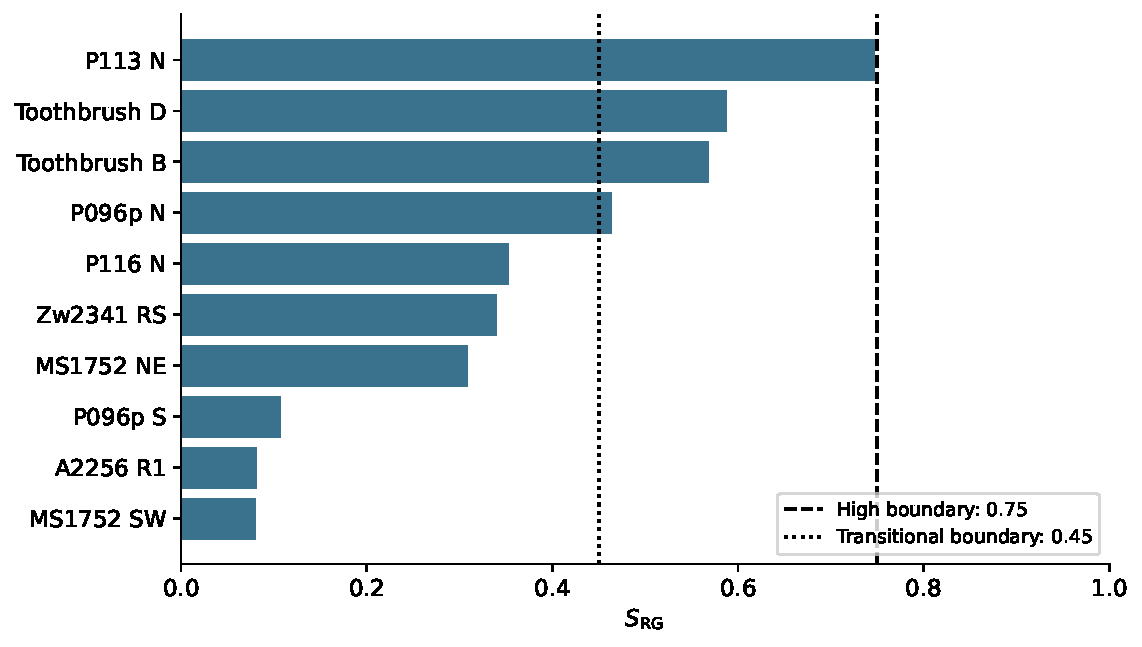
\includegraphics[width=0.9\linewidth]{img/relic_srg_bars.pdf}
\caption[Similarity scores for selected radio relics]{Similarity scores for the ten relics. Dashed and dotted lines mark the high and transitional boundaries, respectively.}
\label{fig:relic_srg}
\end{figure}

For Zw2341 RS, almost all probability lies in \(G\), yet uncertainty and disagreement among members reduce the final score. Conversely, A2256 R1 receives a confident and consistent Spirals assignment, which places it in \(N\) and gives a low score. These examples show how low scores can arise either from weaker reliability within the target groups or from concentrated support for a non-target class (Table~\ref{tab:relics}).

The retained arcs and elongated ridges can receive radio-galaxy-like assignments despite their different physical origin. The range of outputs demonstrates why neither high \(P_\mathrm{RG}\) nor low \(S_\mathrm{RG}\) alone identifies a relic. This visually selected sample does not establish relic-detection completeness or out-of-distribution performance, and the results remain conditional on the manual isolation and clipping of diffuse emission.
